\documentclass[letterpaper, 11pt]{article}
\usepackage{graphicx}
\usepackage{natbib}
\usepackage[left=3cm,top=3cm,right=3cm]{geometry}
\usepackage{parskip}


\renewcommand{\topfraction}{0.85}
\renewcommand{\textfraction}{0.1}

\title{RJObject Paper}
\author{Brendon J. Brewer}

\begin{document}
\maketitle
\abstract{This is the abstract.}

\section{Introduction}
\setlength{\parindent}{0cm}
\setlength{\parskip}{3mm}
Many inference problems have the following structure. There is some unknown
number, $N$, of objects in a region. Each of the $N$ objects has a property
$x$, which may be a single scalar value (for example, a mass), or a set of
values (e.g. a position and a mass).

We would like to assign a prior to the objects' properties $\{x_i\}_{i=1}^N$.
Since $N$ may be large, it is usually easier to assign an ``interim prior''
conditional on some hyperparameters $\alpha$, and then assign a prior to
$\alpha$. This kind of model is usually called {\it hierarchical}.

The prior for $N$, $\alpha$, and $\{x_i\}$ is usually factorised
in the following way:

\begin{eqnarray}
p(N, \alpha, \{x_i\}) &=& p(N) p(\alpha | N) p(\{x_i\} | \alpha, N) \\
&=& p(N) p(\alpha) \prod_{i=1}^N p(\{x_i\} | \alpha).
\end{eqnarray}

Here we have assumed the priors for $N$ and $\alpha$ are independent, and
the interim prior for $\{x_i\}$ is iid and does not depend on $N$.


In other studies, it has been common to do separate runs of Nested Sampling
with different values of $N$. Then, the posterior for $N$ can be calculated
based on the estimates of the evidence or marginal likelihood. Our motivation
for using Nested Sampling is different. With reversible jump MCMC it is possible
to obtain the posterior for $N$ with a single run. However, the exploration
of the posterior may be very difficult, and sometimes the problem may even
contain a phase transition. We use Nested Sampling to overcome these
difficulties.

%%%%%%%%%%%%%%%%%%%%%%%%%%%%%%%%%%%%%%%%%%%%%%%%%%%%%%%%%%%%%%%%%%%%%%%
% Consider having a section on what kind of ME constraint would lead  %
% to the same prior as a hierarchical model.                          %
%%%%%%%%%%%%%%%%%%%%%%%%%%%%%%%%%%%%%%%%%%%%%%%%%%%%%%%%%%%%%%%%%%%%%%%


\section{Sinusoidal Example}
Phase transition

The model for the signal is
\begin{eqnarray}
\mu(t) &=& \sum_{i=1}^N A_i \sin \left(\frac{2\pi t}{T_i} + \phi_i\right)
\end{eqnarray}
where there are $N$ sinusoids in the signal, the
amplitudes are $\{A_i\}$, the periods are $\{T_i\}$, and the phases are
$\{\phi_i\}$.

The sampling distribution (probability distribution for the data given the
parameters) is a normal (gaussian) distribution with mean zero and standard
deviation $\sigma$, applied independently to each data point:
\begin{eqnarray}
y_i | N, \{A_i\}, \{T_i\}, \{\phi_i\} \sim
\mathcal{N}\left(\mu(t_i), \sigma^2\right).
\end{eqnarray}
We simulated some data based on the assumption $N=2$.
The simulated data is shown in Figure~\ref{fig:sinewave_data}, and shows a
large, low period oscillation with a smaller, much faster oscillation
superimposed. The noise level is such that the fast oscillation is difficult
to detect.

\begin{figure}
\begin{center}
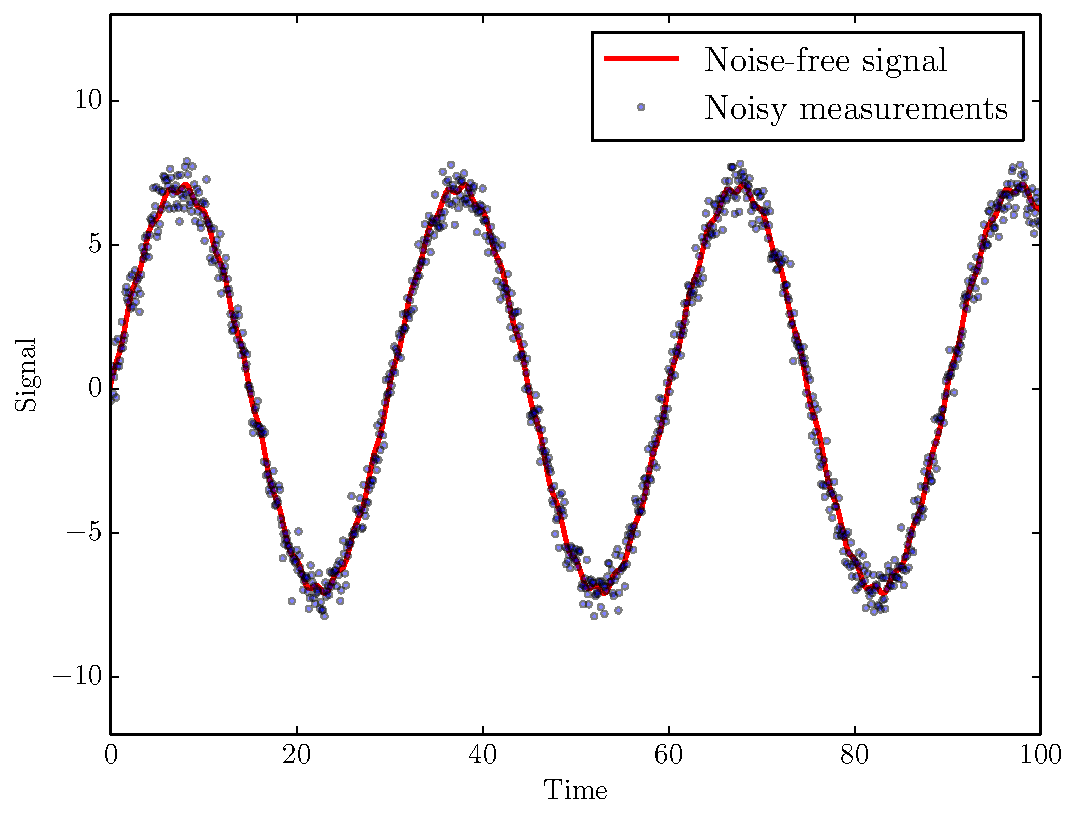
\includegraphics[scale=0.5]{sinewave_data.pdf}
\caption{The simulated data for the sinusoidal example.
\label{fig:sinewave_data}}
\end{center}
\end{figure}


%\section{``Transit'' Example}
%\section{``Asteroseismology'' Example}
%\section{``Galaxy Field'' Example}




\section*{Acknowledgements}
This work is supported by a Marsden Fast-Start grant
from the Royal Society of New Zealand. I would like to thank the following
people for valuable conversations and inspiration:
Anna Pancoast (UCSB), David Hogg (NYU), Daniel Foreman-Mackey (NYU),
Courtney Donovan (Auckland), Tom Loredo (),
John Skilling (MaxEnt Data Consultants), and Daniela Huppenkothen ().


\begin{thebibliography}{}
\bibitem[\protect\citeauthoryear{Brewer, P{\'a}rtay,
\& Cs{\'a}nyi}{2011b}]{dnest} Brewer B.~J., P{\'a}rtay L.~B., Cs{\'a}nyi G., 2011,
Statistics and Computing, 21, 4, 649-656. arXiv:0912.2380

\bibitem[Brewer et al.(2011)]{2011MNRAS.412.2521B} Brewer, B.~J., Lewis,
G.~F., Belokurov, V., Irwin, M.~J., Bridges, T.~J., Evans, N.~W.\ 2011.\
Modelling of the complex CASSOWARY/SLUGS gravitational lenses.\ Monthly
Notices of the Royal Astronomical Society 412, 2521-2529

\bibitem[\protect\citeauthoryear{Green}{1995}]{rjmcmc}
Green, P.~J., 1995, Reversible Jump Markov Chain Monte Carlo Computation and Bayesian Model Determination, Biometrika 82 (4): 711–732.

\bibitem[Neal(2001)]{neal} Neal, R.~M., 2001, 
Annealed importance sampling, Statistics and Computing, vol. 11, pp. 125-139.

\bibitem[\protect\citeauthoryear{Skilling}{1998}]{massinf}
Skilling J., 1998, Massive Inference and Maximum Entropy, in Maximum Entropy
and Bayesian Methods, Kluwer Academic Publishers, Dordrecht/Boston/London p.14

\bibitem[\protect\citeauthoryear{Skilling}{2006}]{skilling} Skilling, J., 2006, Nested Sampling for General Bayesian Computation, Bayesian Analysis 4, pp. 833-860.


\end{thebibliography}

\end{document}

